 
\section{Imaging and Tracking Payload Unit}
\label{sec:changes_itpu}

Design changes were made to the ITPU circuit to include the communication and telemetry modules.

The \ac{ITPU} is implemented on a \acl{TI} \ac{BB} providing onboard processing capabilities and electrical interfaces. Figure \ref{fig:itpu_setup} shows the \ac{ITPU} connection setup to the \ac{E-TAG}. Figure \ref{fig:itpu_pcb} shows the \ac{ITPU} \ac{PCB} top and bottom view which was designed to be tightly stacked to the main header of the \ac{BB} and mounted using nylon screws.
%
\begin{figure}[h!]
\begin{centering}
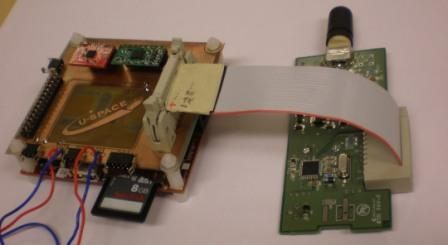
\includegraphics[height=0.25\textheight]{figures/itpu-setup.jpg}
\par\end{centering}
\caption{Setup of the ITPU consisting of the BeagleBoard, the E-Tag and the expansion board with sensors}
\label{fig:itpu_setup}
\end{figure}
%
%
\begin{figure}[h!]
\begin{centering}
\subfloat[Top]{\begin{centering}
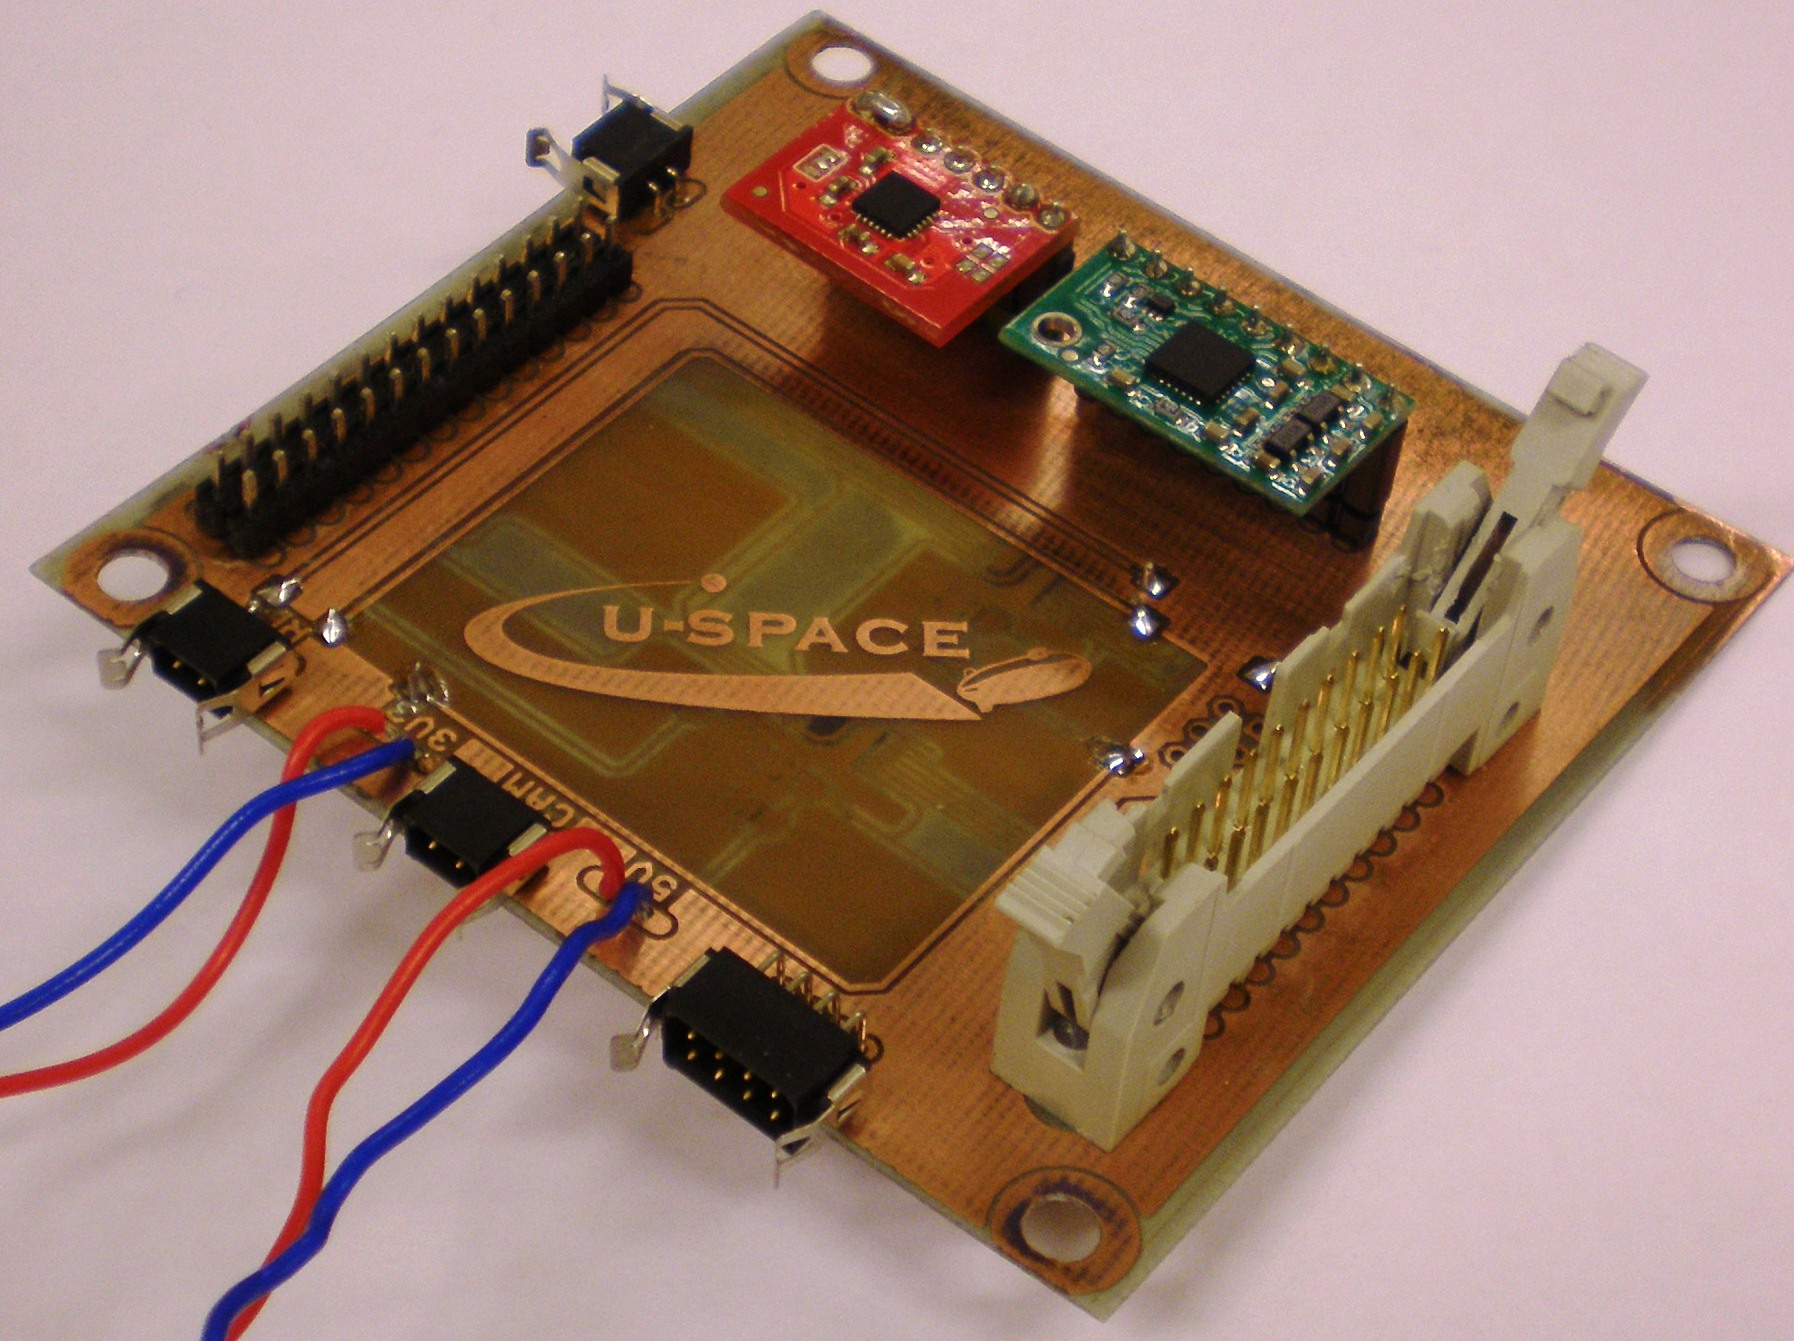
\includegraphics[height=0.25\textheight]{figures/LVC_top.JPG}
\par\end{centering}

}\subfloat[Bottom]{\begin{centering}
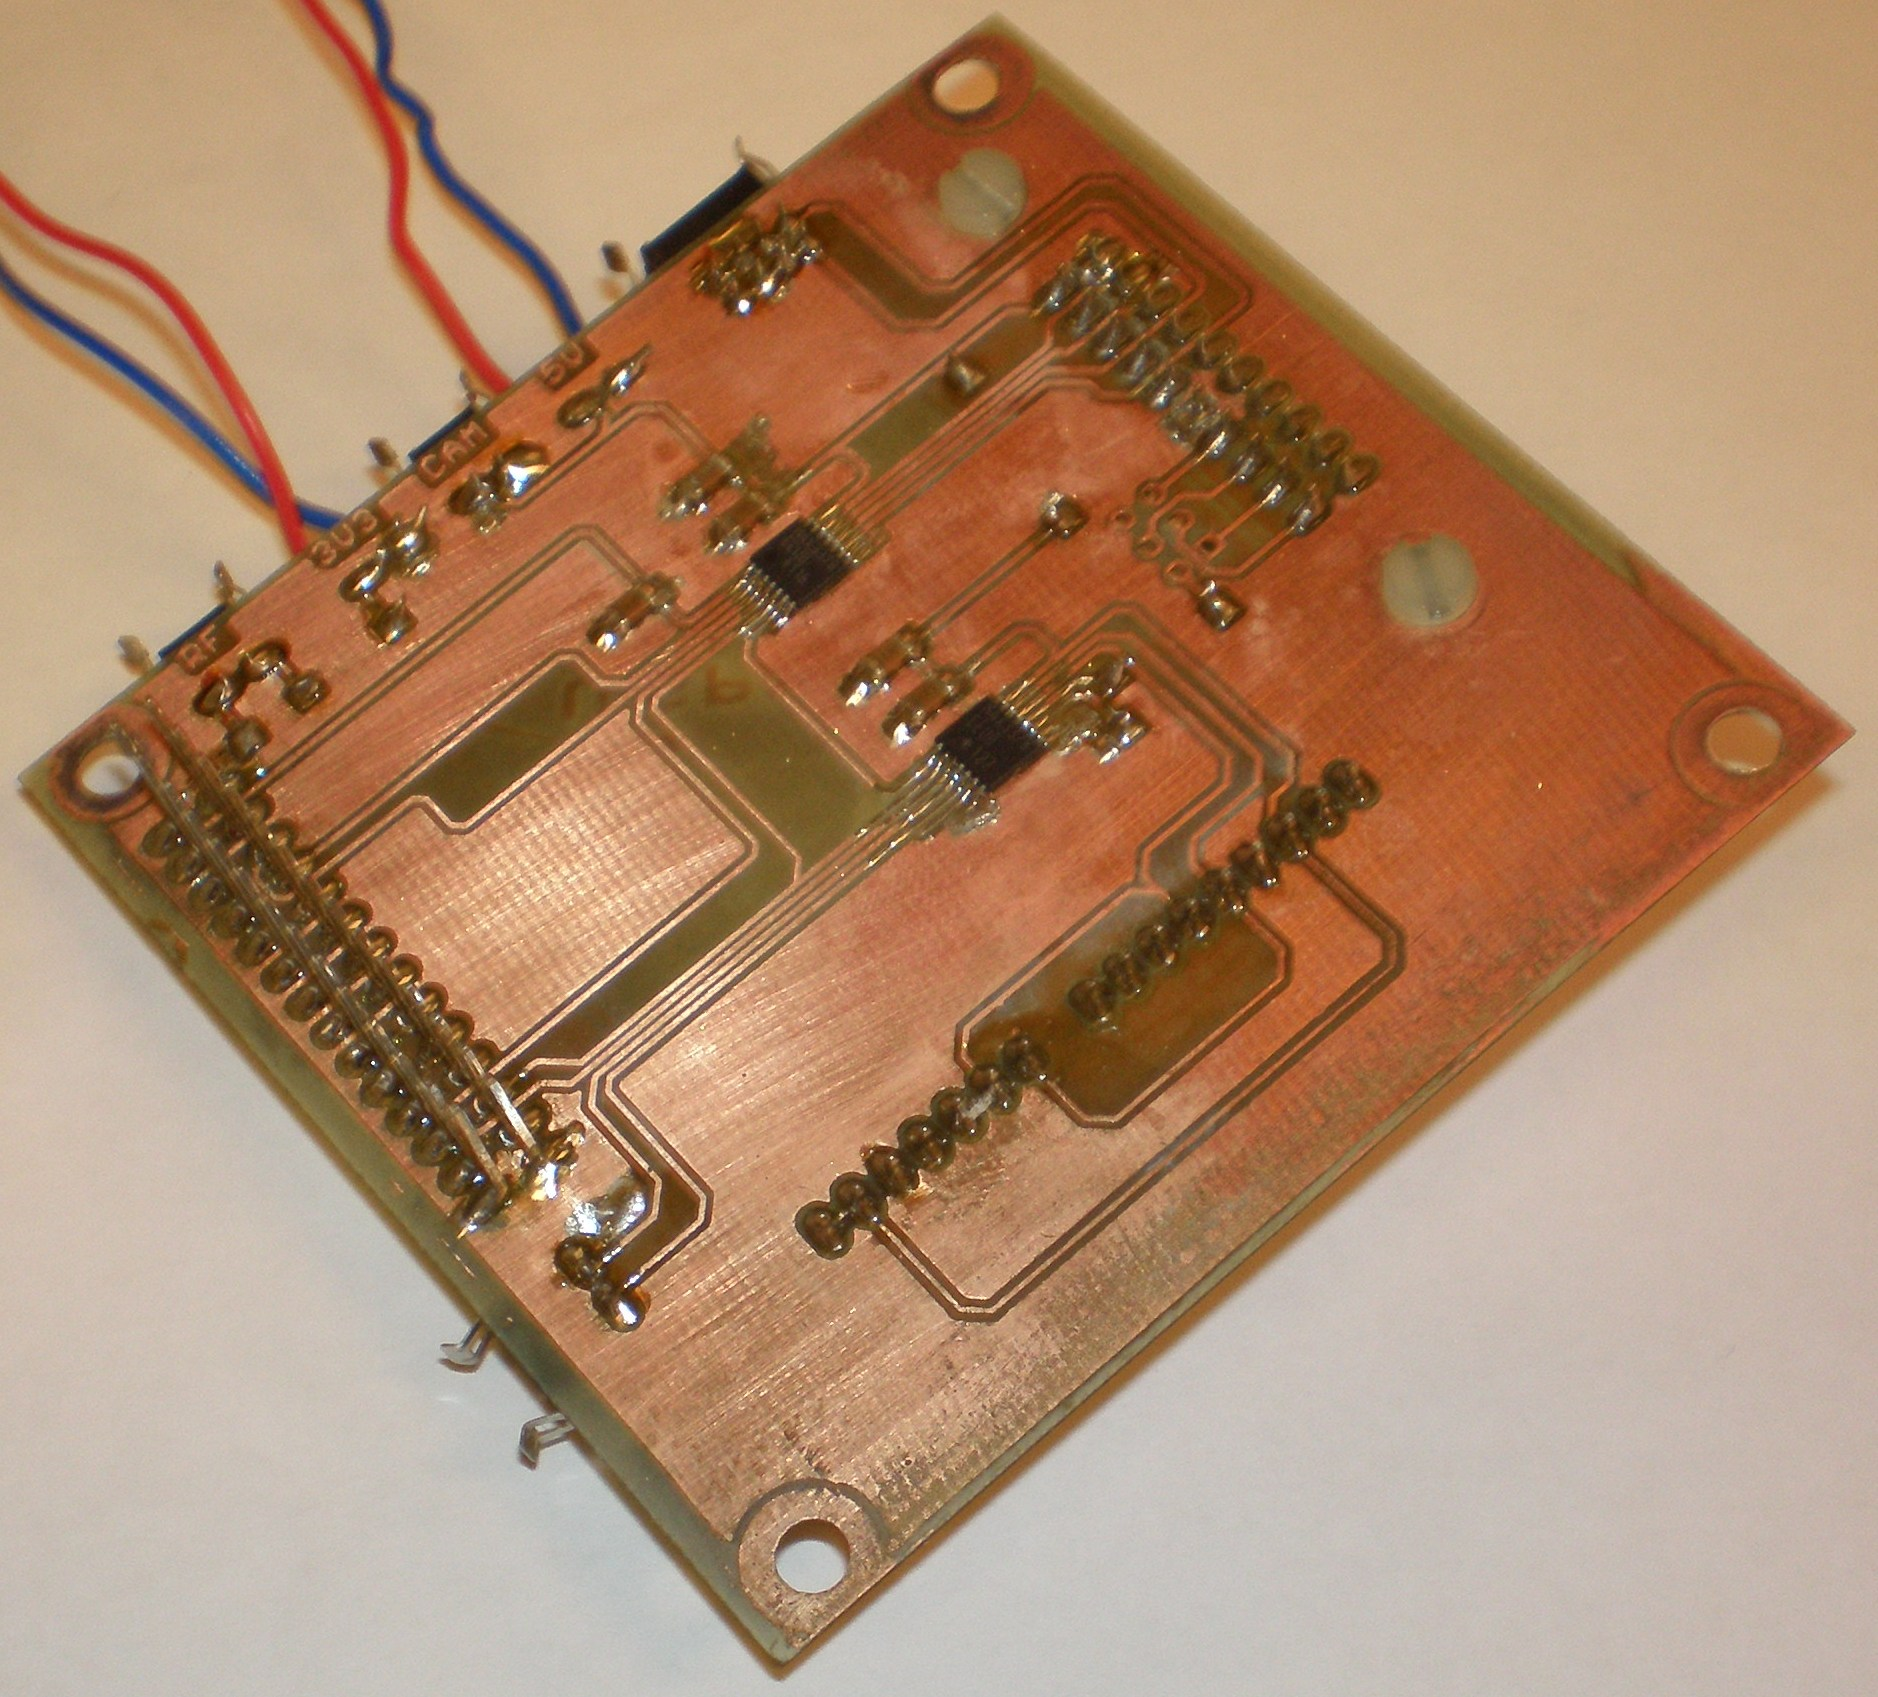
\includegraphics[height=0.25\textheight]{figures/LVC_bottom.JPG}
\par\end{centering}

}
\par\end{centering}
\caption{Populated expansion PCB of the ITPU}
\label{fig:itpu_pcb}
\end{figure}

The main expansion header of the \ac{BB} only provides one \ac{UART} access which is used for \ac{E-TAG} communication. Another \ac{BB} UART was connected to the supplementary expansion header on J4, converted to 3.3~V and connected via wires to the X-Bee telecommunication board. The \ac{I2C} interface was initially only planned to be converted from 1.8~V \ac{BB} level to 3.3~V for the attitude sensors. However, the telemetry conversion module (see \ref{sec:telemetryConv}) required a level shifter to 5~V for the ADCs. 

Both attitude sensor and telemetry system were stable when operating separately, but unstable when operated in parallel on the same I2C-bus. As this was thought to be related to the multiple voltage level shifts, it was tried to use an additional I2C-bus on pins J4 and J5 of the \ac{BB} expansion header. However, the 2nd I2C-bus could not be activated on the BB rev.C4 used for the initial design.
On the software side, the integration of the telemetry and communication system together with the attitude determination and imaging system needed only minor additions to the code base to provide interfaces for communication between both systems. 

A major issue and cause for big changes compared to the CDR was the sudden failure of the BB between the pre-flight test and the scheduled flight-test. No replacement board of the same kind could be acquired on such a short notice so a provided BB-xM was made to fit into the already designed and built system. Although the BB-xM is in general pin-compatible to the BB rev.C4, a problem was the direction of the main expansion header. In the initial BB, the female-header was mounted on the top side of the BB, hence the ITPU-PCB was designed to directly stack on top of the BB. The expansion header of the BB-xM was mounted to the bottom side. Therefore, a direct connection between the two boards was no longer possible. Instead, a ribbon cable was produced but this could not provide a fully stable connection between the BB-xM and the expansion board. However, on the BB-xM it was possible to enable the second I2C-bus on the J4 and J5 expansion headers.
